\documentclass[letterpaper,11pt]{article}
\oddsidemargin -1.0cm \textwidth 17.5cm

\usepackage[utf8]{inputenc}
\usepackage[activeacute,spanish, es-lcroman]{babel}
\decimalpoint
\usepackage{amsfonts,setspace}
\usepackage{amsmath}
\usepackage{amssymb, amsmath, amsthm}
\usepackage{comment}
\usepackage{float}
\usepackage{amssymb}
\usepackage{dsfont}
\usepackage{anysize}
\usepackage{multicol}
\usepackage{enumerate}
\usepackage{graphicx}
\usepackage[left=1.5cm,top=1.5cm,right=1.5cm, bottom=1.7cm]{geometry}
\setlength\headheight{1.5em} 
\usepackage{fancyhdr}
\usepackage{multicol}
\usepackage{hyperref}
\usepackage{wrapfig}
\usepackage{subcaption}
\usepackage{siunitx}
\usepackage{cancel}
\pagestyle{fancy}
\fancyhf{}
\renewcommand{\labelenumi}{\normalsize\bfseries P\arabic{enumi}.}
\renewcommand{\labelenumii}{\normalsize\bfseries (\alph{enumii})}
\renewcommand{\labelenumiii}{\normalsize\bfseries \roman{enumiii})}

\begin{document}

\fancyhead[L]{\itshape{Facultad de Ciencias F\'isicas y Matem\'aticas}}
\fancyhead[R]{\itshape{Universidad de Chile}}

\begin{minipage}{11.5cm}
    \begin{flushleft}
        \hspace*{-0.6cm}\textbf{FI1100 Introducción a la Física Moderna}
    \end{flushleft}
\end{minipage}

\begin{picture}(2,3)
    \put(366, -10){
\includegraphics[scale=0.9]{Imágenes/logo/dfi-fcfm.pdf}}
\end{picture}

\begin{center}
	\LARGE\textbf{Interferencia y Difracción}
\end{center}

\begin{enumerate}\setlength{\itemsep}{0.4cm}

\rfoot[]{pág. \thepage}

\item 
\begin{multicols}{2}
 Dos antenas de radio separadas 300 m transmiten simultáneamente señales idénticas a la misma longitud de onda. El radio en un automóvil que se desplaza al norte recibe estas señales. \textbf{a)} Si el vehículo se encuentra en la posición del segundo máximo, ¿cuál es la longitud de onda de las señales? \textbf{b)} ¿Cuánto más lejos debe viajar el auto para encontrar el siguiente mínimo en recepción? (Nota: No utilice la aproximación de ángulo pequeño en este problema.)

    \columnbreak
    
    \begin{figure}[H]
        \centering
        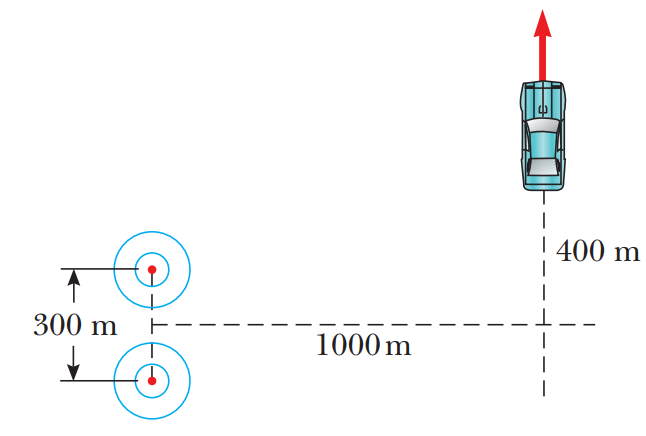
\includegraphics[width=0.75\linewidth]{Imágenes/clases/auto.png}
    \end{figure}
\end{multicols}

\item Considere que una lámina de plástico transparente, de índice de refracción $n$ y espesor $t$, se coloca entre la ranura superior y la pantalla con orientación tal que la luz pasa a través del plástico perpendicularmente a sus superficies, como se muestra en la figura:

\begin{multicols}{2}
    \begin{enumerate}
        \item Cuando se hace esto, el máximo central del patrón de interferencia se mueve hacia arriba en la pantalla en una distancia $y'$. Determine una expresión para la distancia $y'$ en términos de $d, L, N \text{ y } t$
    
        \item Ahora suponga que no se conoce el espesor de la lámina, pero sí se sabe que el rayo de luz tiene longitud de onda $\lambda$. Si el punto central de la pantalla es un punto oscuro en lugar de un punto brillante, ¿cuál es el grosor mínimo de la lámina de plástico?
    \end{enumerate}
    \columnbreak
    \begin{figure}[H]
        \centering
        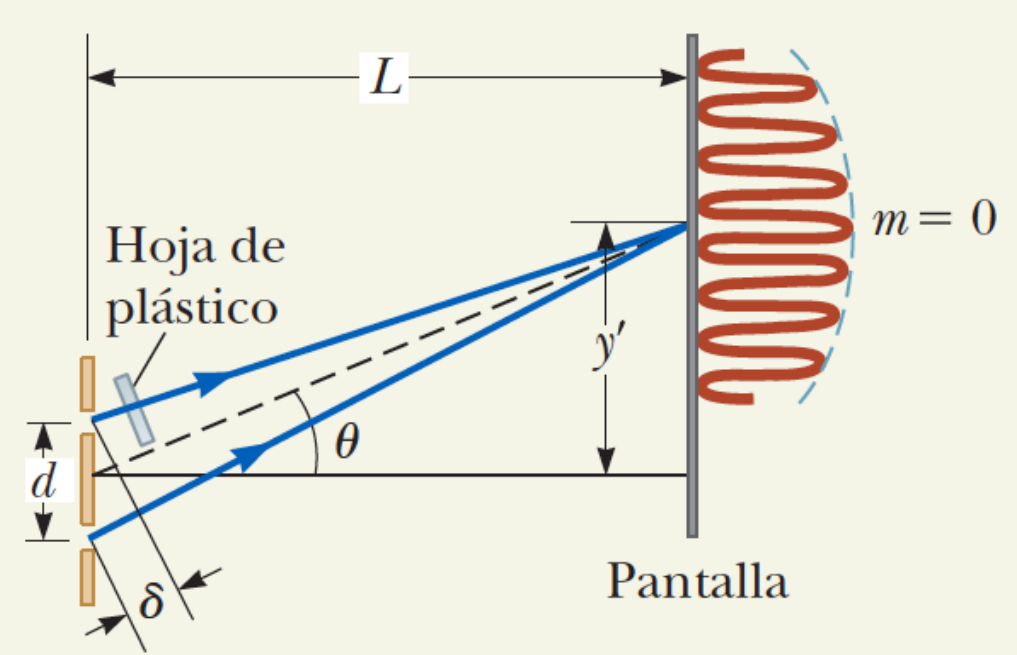
\includegraphics[width=0.9\linewidth]{Imágenes/tutorias/imagen_2023-10-12_144956321.png}
    \end{figure}
\end{multicols}

\item 
\begin{enumerate}
    \item Se observa que en una rendija de apertura $a=\SI{0.8}{\mm}$ ocurre difracción de tal manera que la segunda franja brillante está a una distancia $y=\SI{1.40}{\mm}$ del centro. Si la pantalla está a una distancia $L=\SI{80}{\cm}$, determine la longitud de onda de la luz incidente.

    \item Determine el ancho angular del espectro visible en el primer y tercer orden  que produce una rejilla plana de $600$ ranuras por milímetro cuando incide luz blanca en dirección normal. Considere que las longitudes de ondas del espectro visible abarcan desde $\SI{400}{\nm}$ hasta $\SI{700}{\nm}$
\end{enumerate}

\end{enumerate}
\end{document}